%!TEX root = linear-algebra.tex
\stepcounter{lecture}
\setcounter{lecture}{1}
\pagebreak
\section{Introduction}
 \lecturemarker{0}{ 10.10.2014}



\begin{example}
Consider the definiton of the exponential function: \vspace{-10pt}

\begin{align} \nonumber
exp(x) &= 1 + x + \frac{1}{2}x^2 + \frac{1}{6}x^3 + \dots && \vspace*{5pt}\\\nonumber
&= \sum_{n=0}^{\infty} \frac{x^n}{n!} &&
\end{align}

So $e^{100} = 1 - 100 + \frac{1}{2}100^2 - \frac{1}{6}100^3 + \dots \approx 0$\\

\textit{Is this really true?}\\
Yes, but this is not obvious. The series converges (i.e. tends to an answer) for all $x$. We will see this later...\\
\end{example}

\begin{example}
$f = \dfrac{4}{3+\cos x}$\\

Can we write the power series $f = a_0 + a_1 x + a_2 x^2 + \dots = \sum a_n x^n?$ where $a_n$ are known constants?\\

Yes, we find (somehow) that $f = 1 + \frac{x^2}{8} + \frac{x^4}{192} + \dots$\\

Does this series converge? Using Maple to find the series and plotting $f - \sum_0^{200} a_n x^n$, we actually find that at $\pm 3.60$ish, the difference is non-zero and it fails to converge. This is (apparently) amazing evidence of the existence of the complex plane...\\

\end{example}

\begin{example}
Limits\\

$\displaystyle{\lim_{x \to \infty} (\sin x) = ? }$, it is undefined.\\

$\displaystyle{\lim_{x \to \infty} \left(\dfrac{\sin x}{x}\right) }= 0 $, from the sandwich theorem as 0 is squeezed between $\frac{1}{x}$ and $-\frac{1}{x}$\\\\

$\displaystyle{\lim_{x \to \infty} \left(\dfrac{1}{x\sin x}\right) = ? }$, undefined once more, since whenever $x = n\pi$, the denominator is 0.\\\\

$\displaystyle{\lim_{n \to \infty} \left(\frac{\sin n}{n}\right) }$, $n \in \R$ is not at all obvious (depends on how well you can approximate $\pi$)\\
\end{example}

Clearly we have work to do....



%%%%%%%%%%%%%%%%%%%%
%Actual lectures

\pagebreak


\section{Functions}   \marginnote{Lecture 1\\ 14.10.2014}[-1cm]
       
A function takes an ``input'' and gives a \textbf{unique} output: $f(x) : x \in \mathbb{R}.$\\$f(x)$ is the output or function value at $x$.\\

$f:\mathbb{R} \rightarrow \mathbb{R}$ (alternative notation: $f$ ``maps'' input $\in \mathbb{R}$ to output $\in \mathbb{R}$)

$f$ may not be defined for all reals. A function \textit{should} be defined along with the \textbf{domain} of values over which it applies, e.g.:\\

$f(x) = \sqrt{x^2 -1}$ for $ x \geq 1$\\

Notation: $[a,b] \; \text{means } \forall x : \; a \leq x \leq b \qquad$
$(a,b) \; \text{means } \forall x : \; a < x < b$ \\
These are called \textbf{closed} and \textbf{open} intervals respectively. 

\begin{itemize}
\item[-] So $x \geq 1$ could be written as $x \in [1,\infty)$\\
By convention $\infty$ is never a closed interval since it is not a real number.\\
\end{itemize}


We also define the \textbf{range} of a fucntion to be the set of possible values $f(x)$ as it takes values of the domain.
So $f(x) = \sqrt{x^2 -1 }$ in $[1,\infty)$ has the \textbf{range} $[0,\infty)$.\\

Note: $\sqrt{}$ is always positive conventionally, otherwise it maps to more than one value $\implies f$ is not a function. Hence $\sqrt{x^2} = |x|$, \textit{not necessarily $x$.}\\


\subsektion{How might we define functions?}

\begin{enumerate}
\item An explicit formula\\
 e.g. $f(x) = x^2\sin(x)$\\
(as the domain is not given, we assume it applies for all $x$ or all sensible $x$.)

$f(x) = \dfrac{x+2}{x-1} \qquad$ ``sensible'' here means $x \neq 1$\\

\item Split ranges, e.g.\\

$f(x) = \begin{cases}
 x \text{ if } x > 1\\
 \sin(x^2) \text{ if } 0 < x \leq 1\\
 e^x \text{ if } x \leq 0
 \end{cases}$\\
 
\pagebreak
 
\item As a solution to an equation\\
e.g. $f'' + x^2f = 0, f(0) = 1, f'(0) = 0$ \textit{may} define a function
 
Similarly we could define $f(x) = \displaystyle{\int_0^x t^t \, \mathrm{d}t}$\\(Note: we use a different letter for the \textit{dummy} variable, $t$)\\

\item In words\\
 e.g. $f(x) =$ ``the maximum amount by which $x$ exceeds an integer for $ n = 1,2,...100$''\\

\item An implicit definition\\
 e.g. $f(x)$ given by $f(x) + \frac{1}{2}\sin[f(x)] = x$

(or $y + \sin y = x :$ we can't solve for $y$ in terms of $x$ easily) given $x$, not easy to calculate $f(x)$\\

\item As a limit \vspace{5pt}\\ 
 e.g. $x^{x^{x^{ \udots }}}$ or more formally: $f_1 = x^x$, $f_{n+1} = x^{f_n}$ for $n \geq 1$

If this process tends to a limit as $n \to \infty$ we may have defined a function.
\end{enumerate}

... And so on. There are lots of ways of defining functions. \\

How many functions are there? 

It turns out it's (a very large\footnote{see M1F, there are different sizes of ``infinities''}...) infinity\\

Most functions are \sout{horrible} horrendous.
Even ones which look nice can be nasty...\\

\begin{example} $f(x) = \begin{cases}
 \sin(\frac{1}{x}) & x \neq 0\\
 0 & x = 0
 \end{cases}$\\
 
 \end{example}

The graph crosses the $x$-axis an infinite number of times between $[0,n]$\\

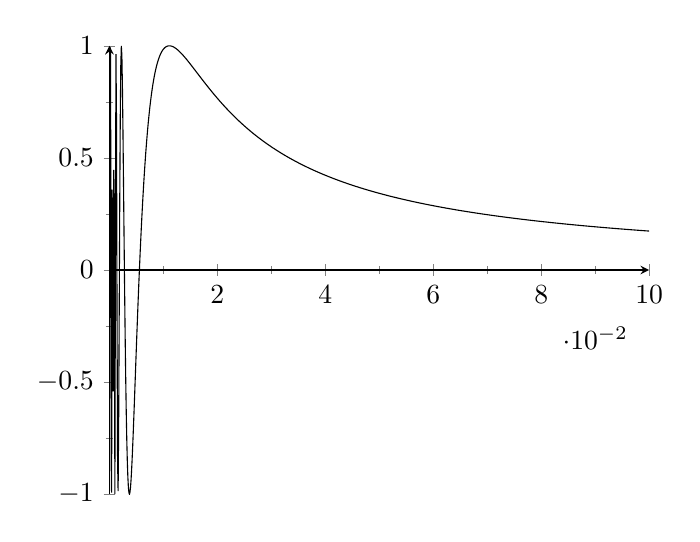
\begin{tikzpicture}
\begin{axis}[
minor tick num=1,
axis y line=left,
axis x line=middle,
]
\addplot[
black,
domain=0.00001:0.1,
samples=1000,
]
{(sin(1/x)};
\end{axis}
\end{tikzpicture}

\pagebreak

\begin{example} $f(x) = e^{-\frac{1}{x^2}}$\\\\

\hvFloat[%
floatPos=htb,%
capWidth=0.5,% of \columnwidth
capPos=r,%
capVPos=c,%
objectPos=c]{figure}{
\tikz{\begin{axis}[
minor tick num=0,
axis y line=middle,
axis x line=middle,
ejes=-10:10 0:1
]
\addplot {exp(-1/x^2)};
\addplot [dash pattern=on 4pt off 4pt] {1};
\end{axis}}
}%
[Caption beside object and vertically centered]{$f(x)$ is so flat at zero that the Macluarin (Taylor) Series converges to 0. This is NOT the right answer. We then call this a non-analytical function.}{fig:1}
\end{example}

\begin{example} $f(x) = \displaystyle{\sum_{n=1}^{\infty} } \dfrac{\sin (n^4x)}{n^2} = \sin x + \dfrac{\sin 16x}{4} + \dfrac{\sin 81x}{9} + \dots$\\

This function is continous everywhere, differentiable nowhere.\\
\end{example}



\subsektion{Inverse functions} \marginnote{Lecture 2\\ 16.10.2014}[-1cm]

Suppose we have a function $f$\\

%%%%%%%%%%%%%%%%%%%%%%
\begin{tikzpicture}
%% Blob
\filldraw [fill=blue!20, draw=blue!60] (0,0) to [quick curve through={(0,0) (.85,1) .. (1,1) .. (.3,2) .. (-1,-2)}] (0,0) ;
\begin{scope}[xshift=2cm, yshift=-1cm]
\filldraw [fill=red!20, draw=red!60] (0,0) to [quick curve through={(0,0) (1,2) .. (2,2) .. (3,2) .. (2,0)}] (0,0) ;
\end{scope}

% the texts
   \node at (-1,0) {$x$};
    \node at (4,0) {$f(x)$};
    \node at (-.7,-2.5) {Domain $f$};
    \node at (4.5,-2.5) {Range of $f$ (also known as image of $f$)};

    % the points in the sets (here I just create nodes to use them later on to position
    % the circles and the arrows
    \node[anchor=east] (x1) at (-1,0.7) {};
    \node[anchor=east] (x2) at (-1.3,-0.7) {};
    \node[anchor=east] (y1) at (3.5,0.5) {};
    \node[anchor=east] (y2) at (3.8,-0.5) {};

    % position the elements in the sets (at the nodes we just created)
    \fill[blue] (x1) circle (1pt);
    \fill[blue] (x2) circle (1pt);
    \fill[red] (y1) circle (1pt);
    \fill[red] (y2) circle (1pt);

    % draw the arrows
    \draw[-latex] (x1) to[out=45,in=120,looseness=1] (y1);
    \draw[-latex] (y2) to[out=220,in=300,looseness=1] (x2);

\end{tikzpicture}
%%%%%%%%%%%%%%%%%


\begin{Definition}\begin{shaded}If it is possible to find a function $g(f(x)) = x \quad \forall x$ in domain of $f$, then $g$ is called the \underline{inverse} of $f$. It's often denotes as $f^{-1}$.
 \end{shaded}\end{Definition}

The domain of $f$ = the range of $f^{-1}$\\
$\&$ The range of $f$ = the domain of $f^{-1}$\\

\textit{Do inverses always exist?} \\
Clearly not if ($\geq$) two $x$ values give the same value of $f(x) = y$ say. As we cannot determine a unique $x$ value given $y$.\\

In practice, we try to solve $f(x) = y$ for $x$. This may find the inverse or tell us that there is a problem.\\

\begin{example} Find the inverse of $f(x) = \dfrac{x-1}{x+3} \qquad (x \neq 3)$\\

$y = \dfrac{x-1}{x+3} \implies y(x+3) = x-1$\\

$\implies x(y-1) = -3y-1 $\\

$\implies x = \dfrac{3y+1}{1-y} = f^{-1}(y)$\\


%%%%%%%%%%%%%%%%%%%%%%%%%%%%%%
\hvFloat[%
floatPos=htb,%
capWidth=0.5,% of \columnwidth
capPos=r,%
capVPos=c,%
objectPos=c]{figure}{ %%%%%% PUT PLOT HERE
\tikz{\begin{axis}[
minor tick num=0,
axis y line=middle,
axis x line=middle,
ejes=-5:-1 -30:30
]
\addplot {(x-1)/(x+3)};
\vasymptote {-3};
\addplot [dash pattern=on 4pt off 4pt] {1};
\end{axis}}
}%%%%% END PLOT THERE
[Caption beside object and vertically centered]{The graph $y = f(x)$ helps us understand what is going on. So we sketch it, noting that $y = \dfrac{x-1}{x+3} = 1 - \dfrac{4}{x+3}$. For inverse to exist, all lines $y$ = constant must intersect $y = f(x)$ \sout{oncee} once and only once, which is clearly the case.
}{fig:1}
%%%%%%%%%%%%%%%%%%%%%%%%%%%%%%

%\tikz{
%\begin{axis}[
%minor tick num=1,
%ejes=-5:-1 -50:50,
%title={$y=f(x+1)=\dfrac{1}{x+1}$}
%]
%    \addplot {(x-1)/(x+3)};
%    \vasymptote {-3}
%    \draw [densely dashed] (axis cs:0,1) -- ({axis cs:0,1}-|{rel axis cs:1,0});
%\end{axis}}

\end{example}



\begin{example} Does $f^{-1}$ exist? for $y = x + \frac{1}{x} = f(x)$\\

Note that if $x = 2$, then $f(2) = 2.5$, but $f(\frac{1}{2}) = 2.5$ also...\\
maybe if we restrict the domain of $f$, we can find a sensible inverse.\\

Lets try $y = x + \frac{1}{x} \implies xy = x^2 + 1$\\

$\implies x^2 - xy + 1 = 0$\\

$\implies x = \dfrac{y \pm \sqrt{y^2 -4}}{2}$\\

Which root should we take? Sketching $f(x)$, we can note that $y = k$ intersects the graph: $\begin{cases}
\text{Not at all}& -2 < k< 2\\
\text{Once} & k = \pm 2\\
\text{Twice} & k>2 \text{ or } k<-2
\end{cases}$



%%%%%%%%%%%%%%%%%%%%%%%%%%%%%%
\hvFloat[%
floatPos=htb,%
capWidth=0.5,% of \columnwidth
capPos=r,%
capVPos=c,%
objectPos=c]{figure}{ %%%%%% PUT PLOT HERE
\tikz{\begin{axis}[
minor tick num=5,
axis y line=middle,
axis x line=middle,
ejes=-4:4 -10:10
]
\addplot {x + 1/x};
\end{axis}}
}%%%%% END PLOT THERE
[Caption beside object and vertically centered]{The graph $y = x + \dfrac{1}{x}$
}{fig:1}
%%%%%%%%%%%%%%%%%%%%%%%%%%%%%%


\vspace{5pt}

Suppose we restrict the domain of $f$ to be $|x| \leq 1$ (exlcluding $x$ =0).\\

Then we can define the inverse function:\\

$f^{-1}(y) = \begin{cases}
 \dfrac{y - \sqrt{y^2 -4}}{2} & \text{ if } y \geq 2 \\\\
 \dfrac{y + \sqrt{y^2 -4}}{2} & \text{ if } y \leq 2 \\

 \end{cases}
 $

If instead we restrict the domain of $f$ to be $|x| \geq 1$ then:
$f^{-1}(y) = \begin{cases}
 \dfrac{y + \sqrt{y^2 -4}}{2} & \text{ if } y \geq 2 \\\\
 \dfrac{y - \sqrt{y^2 -4}}{2} & \text{ if } y \leq 2 \\

 \end{cases}
 $

So a little care is required.\\
\end{example}

\subsubsektion{Trigonometric Functions}

\textbf{Trigonometry:} 
\greektext{τρίγωνον}
\greektext trigōnon metron 
\latintext - The Measuring of Triangles\\


Later we will define $\cos(x), \sin(x), \tan(x),$ but you already know them. \\


\textbf{Inverse Cosine}
If $f(x) = \cos(x)$ then $f^{-1}(x) = \cos^{-1}(x)$ (or $\arccos(x)$) exists for some $x$ and some agreed domain of $f(x)$\\

\begin{figure}[!htb]
\centering
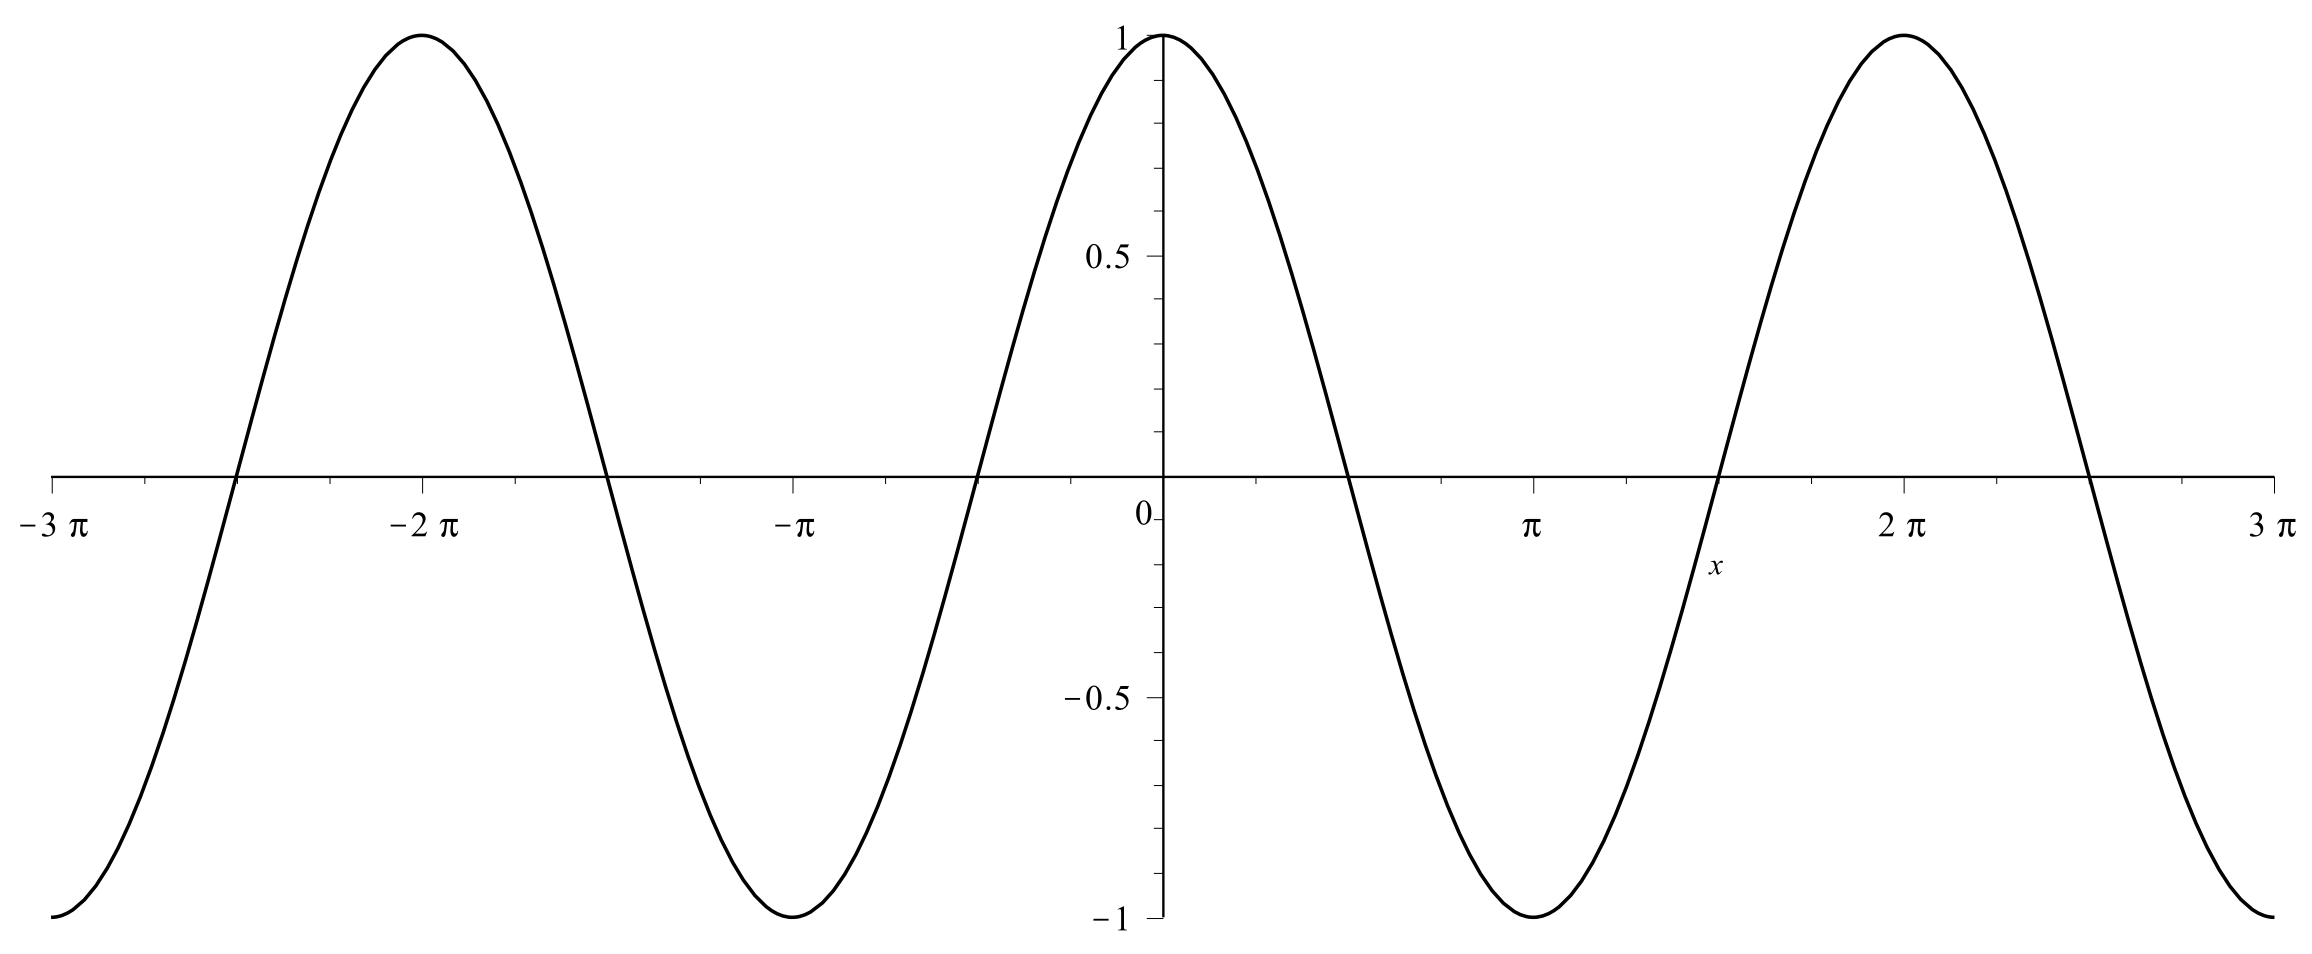
\includegraphics[height=5cm]{cosx.png}
\label{fig:digraph}
\end{figure}

The natural domain to restrict is $0 \leq x \leq \pi$. Then $\cos^{-1}(y)$ exists uniquely, provided $|y| \leq 1$.\\

Now remove the restrictions on $x$. Solve the equation $\cos x = \alpha \qquad $\\

General solution: $\boxed{ x = 2n\pi \pm \cos^{-1}\alpha \quad (n \in \Z)}$\\

But remember $0 \leq \cos^{-1} \leq \pi $ always!\\

\textbf{Inverse Sine}


\begin{wrapfigure}{L}{0.5\textwidth}
  \begin{center}
\tikz{\begin{axis}[
minor tick num=0,
axis y line=middle,
axis x line=middle,
ejes=-6.28359265358:6.28359265358 -2:2
]
\addplot {sin(deg(x))};
\end{axis}}  
\end{center}
\end{wrapfigure}



We restrict $-\frac{\pi}{2} \leq x \leq \frac{\pi}{2}$ i.e. $|x| \leq \frac{\pi}{2}$\\

Then the inverse function $\sin^{-1}y$ exists, if $|y| \leq 1$\\

So $-\frac{\pi}{2} \leq \sin^{-1} \leq \frac{\pi}{2}$\\

Then the equation $\sin x = \beta$ has the general solution:\\

$x = 2n\pi + \sin^{-1}\beta$ if $n$ is even\\
$x = 2n\pi - \sin^{-1}\beta$ if $n$ is odd\\ \vspace{2pt}
$= \boxed{ x = 2n\pi + (-1)^n \sin^{-1}\beta \quad (n \in \Z)}$\\\\

.\\

\textbf{Inverse Tan}\\


%%%%%%%%%%%%%%%%%%%%%%%%%%%%%%
\hvFloat[%
floatPos=htb,%
capWidth=0.5,% of \columnwidth
capPos=r,%
capVPos=c,%
objectPos=c]{figure}{ %%%%%% PUT PLOT HERE
\tikz{\begin{axis}[
minor tick num=0,
axis y line=middle,
axis x line=middle,
ejes=-3.14159265358:3.14159265358 -10:10
]
\addplot {tan(deg(x))};
\vasymptote{3.14159/2};
\vasymptote{-3.1415926/2};
\end{axis}}
}%%%%% END PLOT THERE
[Caption beside object and vertically centered]{ 
We restrict $-\frac{\pi}{2} \leq \tan^{-1}y \leq \frac{\pi}{2}$ defined $\forall y$.
So finally $tanx = \gamma$ has general solution: $\boxed{x = n\pi + \tan^{-1}\gamma}$
}{fig:1}
%%%%%%%%%%%%%%%%%%%%%%%%%%%%%%



\pagebreak

\subsektion{Parity - Even \& Odd Functions} \marginnote{Lecture 3\\ 17.10.2014}[-1cm]
\vspace*{-5pt}
\begin{Definition} \begin{shaded}
A function $f(x)$ defined over a symmetric domain (i.e. $[-a,a]$) is called even $\iff f(-x) = f(x)$ and odd $\iff f(-x) = -f(x)$ \end{shaded}
\end{Definition}

e.g. $x^2$ is even, $\sin x$ is odd. Functions need not be even or odd.\\

But any function (over a symmetric domain) can be written as the sum of an even function \& an odd function. \\

\begin{example}
$\dfrac{x}{x+1} = \dfrac{x}{x+1} \dfrac{(x-1)}{(x-1)} = \dfrac{x^2}{x^2-1} \;-\; \dfrac{x}{x^2-1}$\\
\hspace*{170pt} Even \hspace{15pt} Odd
\end{example}

\begin{example}
$\cos(x+3) = \cos x \cos 3 \; - \; \sin x \sin 3$\\
\hspace*{130pt} Even \hspace{30pt} Odd\\
\end{example}\\

In general, how do we write $f(x) = f_e(x) + f_o(x)$?
\begin{align}
f(x) &= f_e(x) + f_o(x) &&\\ \nonumber
\implies f(-x) &= f_e(-x) + f_o(-x) &&\\
\implies f(-x) &= f_e(x) - f_o(x)
\end{align}

Solving (1) and (2) by adding: \\

$\implies f_e(x) = \frac{1}{2} [f(x) + f(-x)]$\\

and similarly $f_o(x) = \frac{1}{2} [f(x) - f(-x)]$\\

To prove that we can always find these two functions, start again from other way:\\

Define $f_e$ \& $f_o$ as above, note: 
\begin{enumerate}
\item $f_e$ is even
\item $f_o$ is odd
\item $f_e + f_o = f$
\end{enumerate}\\

This proves that any $f$ has an even part and an odd part.\\

\begin{example}
Redo example 6. $f(x) = \dfrac{x}{x+1} = f_e(x) + f_o(x)$\\

$\implies f_e(x) = \frac{1}{2} \left[\dfrac{x}{x+1} + \dfrac{-x}{1-x}\right]$\\

$ = \frac{1}{2} \left[\dfrac{x - x^2 - x^2 -x}{(1+x)(1-x)}\right] = \dfrac{-x^2}{1-x^2} = \dfrac{x^2}{x^2-1}$ as before.\\\\

\end{example}

\subsubsektion{Evaluating Integrals}
Parity is a great help when evaluating integrals.\\

What is $\displaystyle{ \int_{-\pi}^{\pi} \dfrac{x + \sin (x^3)}{1 + e^{x^2}} \, \mathrm{d}x}$?\\

Replacing $x$ by $-x$ we can see that the integrand is an odd function since $f(-x) = -f(x)$ 

Hence the Integral = 0.\\\\ \vspace{50pt}

%%%%%%%%%%%%%%%%%%%%%%%%%%%%%%
%%% Sketch of odd Area A = Area B
%%%%%%%%%%%%%%%%%%%%%%%%%%%%%%

In general $I = \displaystyle{\boxed{\int_{-a}^{a} f_o(x) \, \mathrm{d}x = 0}}$\\

Substituting $t = -x$

\begin{flalign}\nonumber
 \implies I &= \int_{a}^{-a} f_o(-t) \, (\mathrm{-d}x) &&\\ \nonumber
 &=  \int_{-a}^{a} f_o(-t) \, (\mathrm{d}x) \qquad \text{[Use - sign to swap limits]} &&\\\nonumber
 &=  -I &&
\end{flalign}

Hence $I = -I \implies I = 0$.\\

We conclude that if $f(x)$ is odd, then $ \displaystyle{\int_{-a}^{a} f(x) \, \mathrm{d}x = 0}$\\\\

Later we will deal with power series $f(x) = a_0 + a_1x + a_2x^2 + ...$, where $a_i$ is a given constant  for $i \in \N$\\

If $f(x)$ is even then $a_1 = 0, a_3 = 0$ etc., i.e. $a_{odd} = 0$\\
If $f(x)$ is odd then $a_0 = 0, a_2 = 0$ etc., i.e. $a_{even} = 0$\\

So even/odd functions only have even/odd powers of x.\\

\pagebreak


\subsektion{Periodicity}
\begin{Definition} \begin{shaded}
We say a function $f(x)$ is $T$-periodic if and only if $f(x + T) = f(x) \forall x$, where $T >0 $ and $T$ is the smallest value for which this holds.\end{shaded}

\end{Definition}


So although $\sin (x+ 4\pi) = \sin x \; \forall x$, we do not say that $\sin x$ is $4\pi$ periodic, as $\sin (x + 2\pi) = \sin (x) $ as well.\\

\bgroup
\def\arraystretch{1.5}
\begin{table}[H]
    \begin{tabular}{l|l}
    \hline
    $f(x)$            & period                                                    \\ \hline
    $\cos^2x$         & $\pi$                                                     \\
    $\cos |x|$        & $2\pi$                                                    \\
    $|\cos x|$        & $\pi$                                                     \\
    $\sin (\alpha x)$ & $\frac{2\pi}{\alpha} \quad (\alpha \neq 0)$               \\
    $3$                 & depends on definition, say period = 0 \& change definiton \\
    $\sin |x|$        & not periodic                                              \\
    $| \sin x|$       & $\pi$                                                     \\
    \end{tabular}
\end{table}
\egroup

\textbf{Are there any other periodic functions (other than the trigonometric ones)?}\\

%%%%%%%%%%%%%%%%%%%%%%
%%%% 
%%%% Sketch of Random function a to a+L
%%%%
%%%%%%%%%%%%%%%%%%%%%%

We can turn any function into a periodic one.\\
Any function defined on a finite interval can be extended into a periodic function over all $\R$ by copying.\\

Define $f(x + L) = f(x)$ to replicate the behaviour $\forall x$.\\\\


\pagebreak

\subsektion{Polynomials} \marginnote{Lecture 4\\ 21.10.2014}[-1cm]
\vspace*{-5pt}
\begin{Definition} \begin{shaded}
An $n$th order polynomial in $x$ is a function of the form: $f(x) = \displaystyle{\sum_{a=0}^{N} a_n x^n}$ where $a_N \neq 0$\\
$N$ is called the \textbf{degree} or \textbf{order} of the polynomial.. $a_n$ for $n = 0,...,N$ are called the coefficients. If $a_n$ is real $\forall n$, we say the polynomial is real (even if $x$ may be complex).\end{shaded}
\end{Definition}

\begin{theorem}[The Fundamental Theorem of Algebra]

Every polynomial has a root (possibly complex). In general, we call a value $\alpha$ a root of $f(x)$ if $f(\alpha)$ = 0. 

\end{theorem}

\begin{proof}\renewcommand{\qedsymbol}{}
See next year's course M2PM3 on Complex Analysis...\\
\end{proof}

\begin{corollary}
If $c$ is a root of an $N$th order polynomial $P_N(x)$, then we can write $P_N(x) = (x-c)P_{N-1}(x)$.
\end{corollary}

\begin{corollary}
Every $N$th order polynomial has precisely $N$ roots, allowing for repeated roots. e.g. $(x-1)^2$ has roots 1,1.
\end{corollary}

\begin{corollary}
If $P(x)$ is a real polynomial with a complex root $\alpha + i\beta$ ($\alpha, \beta$ real, $\beta \neq 0$), then it also has root $\alpha - i\beta$ (the complex conjugate).
\end{corollary}

\begin{corollary}
Every real polynomial can be written as:\\ $P_N(x) = A(x-r_1)(x-r_2)...(x-r_M)((x-\alpha _1)^2 + \beta ^2)((x-\alpha _2)^2 + \beta _2^2)...((x - \alpha _ L)^2 + \beta _L^2)$\\

Where $r_1.. r_M$ are the real roots, and $(\alpha \pm i \beta),... (\alpha _L \pm i\beta _L)$ are the complex roots and $M + 2L = N$\\

i.e. Any real polynomial can be written as a product of real linear and quadratic factors.\\

N.B. If the polynomial is not real (i.e. if at least one coefficient is strictly complex), then the complex roots need not be in conjugate pairs.\\
\end{corollary}


\subsubsektion{Roots of polynomials}
\begin{itemize}

\item Linear: $ax + b = 0$, one trivial root

\item Quadratic: $ax^2 + bx + c = 0$\\

Formula: $x = \dfrac{-b \pm \sqrt{b^2 - 4ac}}{2a} \quad$ \underline{OR} $\quad x = \dfrac{2c}{-b \pm \sqrt{b^2 - 4ac}}$\\


\textbf{Exercise 1}: Show these are the same. \\
\textbf{Exercise 2}: Use your calculator to solve the equation $\epsilon x^2 + (1 + \epsilon)x + 1 = 0$, where $\epsilon$ is very small (i.e. $10^{-12}$).\\

Subtracting two numbers which are very close together leads to severe accuracy loss c.f. Patriot missiles. The ``Best'' formula to solving a quadratic depends on $a, b$ and $c$ in practice.\\

\item Cubics: $ax^3 + bx^2 + cx + d = 0$

There is a formula\footnote{$x = \sqrt[3]{\left(\frac{-b^3}{27a^3} + \frac{bc}{6a^2} - \frac{d}{2a}\right) + \sqrt{\left(\frac{-b^3}{27a^3} + \frac{bc}{6a^2}-\frac{d}{2a}\right)^2 - \left(\frac{c}{3a}-\frac{b^2}{9a^2}\right)^3}} + \sqrt[3]{\left(\frac{-b^3}{27a^3}+\frac{bc}{6a^2}-\frac{d}{2a}\right) + \sqrt{\left(\frac{-b^3}{27a^3}+\frac{bc}{6a^2}-\frac{d}{2a}\right)^2 - \left(\frac{c}{3a}-\frac{b^2}{9a^2}\right)^3}} - \frac{b}{3a}$},
 but it has very little practical use.\\

\item Quartics: $ax^4 + bx^3 + cx^2 + dx + e = 0$

There is also a general formula... once again not worth knowing\footnote{or even typesetting...}\\

\item Quintics: $ax^5 + bx^4 + cx^3 + dx^2 + ex + f = 0$

There is no general formula to express the roots in terms of radicals. See Galois Theory in 3rd year. But one can easily find the roots in practice for any particular case.\\

\item $N$ > 5: Similarly no formula. However considering general $N$:
\begin{flalign} \nonumber
P_N(x) &= a_Nx^N + a_{N-1}x^{N-1} + \dots &&\\ \nonumber
&= a_Nx^N\left[1 + \frac{a_{N-1}}{a_N} \frac{1}{x} + \frac{a_{N-2}}{a_N} \frac{1}{x^2} + \dots \right]
\end{flalign}


As $\displaystyle{ |x| \to \infty, \frac{1}{x^N} \to 0 }$, So for large $|x|, P_N \approx a_Nx^N$. Hence if $a_N > 0$ WLOG, then as $\displaystyle{x \to \pm \infty , \; P_{2N}(x) \to +\infty \text{ and } P_{2N+1} \to \pm \infty }$\\  
%%%%%%%%%%%%%%%%%%
%
% PUT SKETCH OF POINT HERE

%%%%%%%%%%%%%%%%%
\end{itemize}

\subsektion{Rational Functions} \marginnote{Lecture 5\\ 23.10.2014}[-1cm]

A function of the form $f(x) = \dfrac{P(x)}{Q(x)}$, where $P(x)$ and $Q(x)$ are polynomials is called a rational function.\\ We \textit{could} require that the order of $P < $ order of $Q$. If this doesn't happen, we can use polynomial division to write: 

\[\frac{P}{Q} = R(x) + \frac{S(x)}{Q(x)} \quad \text{ where } R \text{ and } S \text{ are also polynomial}\]\\
\[\text{e.g. } \frac{x^2 + x}{x -1} = \frac{x^2 - x + 2x}{x-1} = x + \frac{2x}{x-1} = x + \frac{2x-2+2}{x-1} = (x+2) + \frac{2}{x-1} \]\\
We could also require that $P$ and $Q$ have no common factors i.e. $\nexists \alpha : P(\alpha) = 0 = Q(\alpha)$ \\
Let's do this! (for simplicity). Any zero of $Q(x)$ is then a \textbf{singularity} or \textbf{pole} or infinity of $\frac{P}{Q}$ and is important. This behaviour is illustrated by...

\vfill
\pagebreak

\subsubsektion{Partial Fraction Decomposition}

Suppose $Q$ has degree $N$, with no repeated root, i.e.

\[Q = \lambda (x-r_1)(x-r_2)\dots(x-r_N) \quad \text{ where } \lambda \neq 0, r_i \neq r=j \text{ unless } i = j \text{ \& } r_i \in \mathbb{C}\]

Then we can write:

\[\frac{P}{Q} = \frac{A_1}{x-r_1} + \frac{A_2}{x-r_2} + \dots + \frac{A_N}{x-r_N} + \overbrace{R(x)}^\text{if needed} \]

We can easily find $A_i$ by multiplying through $Q$:
\begin{align} \nonumber P &= \frac{A_1Q}{x-r_1} + \frac{A_2Q}{x-r_2} + \dots + \frac{A_NQ}{x-r_N}\\ \nonumber
&= A_1 \lambda(x-r_2)(x-r_3)\dots(x-r_N) + \frac{A_2Q}{x-r_2} + \dots + \frac{A_NQ}{x-r_N} \quad (*)
\end{align}

Putting $x = r_1$ into $(*)$; $Q(r_1) = 0$, so:
\[P(r_1) = A_1 \lambda (r_1 - r_2)(r_1 - r_3)\dots(r_1 - r_N) \]

Using the product rule for differentiation, we also now have:
\[
Q'(x) = \lambda[(x-r_2)\dots(x-r_N)] + \lambda(x-r_1)[\text{ a load of stuff }]
\]

So $Q'(r_1) = \lambda(r_1-r_2)(r_1-r_3)\dots(r_1-r_N)$, hence $P(r_1) = A_1Q'(r_1)$ or $A_1 = \dfrac{P(r_1)}{Q'(r_1)}$

So obviously $\boxed{A_i = \dfrac{P(r_i)}{Q'(r_i)} \quad i = 1,2,...,N}$\\\\

\textbf{What could go wrong?}

\begin{itemize}
\item[(a)] \textit{What if (some of) the roots are complex?}\\
Algebra still works. But for some purposes we may prefer to keep things real.
\[ \begin{align} \nonumber \text{e.g.}\quad \frac{3}{x^3+1} = \frac{3}{(x+1)(x^2 - x + 1)} &= \frac{3}{(x+1)(x-\omega)(x+\omega *)} \\ \nonumber
 &= \frac{A_1}{x+1} + \frac{A_2}{x - \omega} + \frac{A_3}{x - \omega *}\\
 \end{align}
\] 

Using the formula we obtained for $A_i$, we get $A_1 = 1, A_2 = -\omega, A_3 = -\omega *$
\[\begin{align} \nonumber \frac{3}{x^3 + 1} &= \frac{1}{x+1} - \frac{\omega}{x-\omega} - \frac{\omega *}{x - \omega *} \\\vspace*{5pt} \nonumber
&= \frac{1}{x+1}  - \frac{x-2}{x^2 - x + 1} \end{align}\]

Alternative Partial Fraction Form for real polynomials:
\[\frac{P}{Q} = R + \frac{A_1}{(x-r_1)} + \dots + \underbrace{\frac{Cx + D}{Cx^2 + \delta x + \delta}}_\text{for complex roots} + \dots \]

\item[(b)] \textit{What if there are repeated roots?}

\end{itemize}

\pagebreak

\chapter{Limits and Power Series} \marginnote{Lecture 6\\ 24.10.2014}[-1cm]


A function of the form $f(x) = \sum_{n=0}^{\infty} a_n x^n$ \\

We wil asume for now that the infinie sum converges (i.e. tends to al imit) for at least some values of $x$. We will also assume we can manipulate infinite series sensibly. The $a_n$ are called cefficients (may be $\in \mathbb{C}$)\\

\pagebreak
\section{Infinite Series}
\subsektion{The Exponential Function}\\

$f(x) = \sum_{n=0}^{\infty} \frac{x^n}{n!} = 1 + x + \frac{x^2}{2} + \frac{x^3}{6} + \dots \quad$In fact this series converges $\forall x$\\

Forget everything we know about $e^x$ for now... What can we deduce about $f(x)$\\

If $x>0, f(x) > 1$ by inspection, and also $x$ increases as $f(x)$ increases.\\

Question 6 on the problem sheets proved that $\forall x,y, f(x)f(y) = f(x+y)$\\

Setting $y = -x$, yields $f(-x) = \frac{1}{f(x)}$, which tells us about when $ 0<x <1$
\begin{itemize}
\item $f(x) \to 0$, as $x \to -\infty$ etc. 
\end{itemize}


It follows that $f(x)$ has an inverse functin $g(x)$ whose domain is $(0,\infty)$ and range $(-\infty,\infty)$, so we know that $x = g(f(x)) \forall x \qquad \& \qquad x = f(g(x)) \; , x>0$\\

Now consider $x^2 = x.x = f(g(x)) .f(g(x)) = f(2g(x))$, obviously by induction $x^n = f(ng(x))$ for $n \in \N$\\

\begin{Definition} \begin{shaded}
I) $x^{\alpha} = f(\alpha g(x)) = e^{\alpha \log x}$ for $x >0,$ any arbitrary $\alpha$\\
\hspace*{55pt} II) $a^x = f(x(g(a))$ for $a > 0$, any abitrary $x$
\end{shaded} \end{Definition}


From the definiton of $f$, $a^x = 1 + x(g(a) + \frac{1}{2} [xg(a)]^2 + \frac{1}{3!}[xg(a)]^3 + \dots$\\

Choose a such taht $g(a) = 1$, then we have:\\
$a^x = 1 + 1 + \frac{1}{2} + \frac{1}{3!} + \dots = 2.718281828459...$\\

Let;s call this value (...wait for it), $e$\\
 Then $g(e) = 1$, so $e^x = \sum_{n=0}^{\infty} \frac{x^n}{n!} = 1 + x + \frac{x^2}{2} + \frac{x^3}{6} + \dots $!!

From now we can use all the properties of the exponential function, e.g. $e^xe^y = e^{x+y}, \quad (e^a)^b = e^{ab}, \quad e^0 = 1$\\

Calling $g(x) = \log(x) = ln(x)$, we have the usual properties which follows from the first problem sheet:\\
\begin{itemize}
\item $\log(uv) = \log(u) + \log(v)$
\item $\log(1) = 0$
\item ``$\log(0)= -\infty$''
\item $\log (\frac{u}{v}) = \log(u) - \log(v)$
\item $\log(a^b) = b\log a$
\item $a^b = e^{b \log a}$
\end{itemize}
(We will not consider logarithms to different bases)\\\\

$e^x$ is defined $x \in R$, \textbf{ what if $x$ is complex or purely imaginary?}\\

Write $x = i\theta, \theta \in R$, then define $e^{i\theta}$ to be:\\

$f(i \theta) = \sum_{n=0}^{\infty} \frac{(i\theta)^n}{n!} = 1 + i\theta + \frac{1}{2}(i\theta^2 + \frac{1}{3!}(i\theta)^3 + \frac{1}{4!}(i\theta)^4 + \dots$\\

$ = (1 - \frac{1}{2}\theta^2 + \frac{\theta^4}{4!} - \frac{\theta^6}{6!} + \dots) + i(\theta - \frac{\theta^3}{3!} + \frac{\theta^5}{5!} + \dots)$\\

Now define $coz(\theta) = (1 - \frac{1}{2}\theta^2 + \frac{\theta^4}{4!} - \frac{\theta^6}{6!} + \dots)  $ and $zin(\theta) = (\theta - \frac{\theta^3}{3!} + \frac{\theta^5}{5!} + \dots) $\\

We then have: $\boxed{e^{i\theta} = coz(\theta) + izin(\theta)}$\\\\\vspace{15pt}


\marginnote{Lecture 7\\ 28.10.2014}[-1.5cm]

A better proof that $coz(x+y) = coz(x)coz(y) - zin(x)zin(y)$ (see appendix for series proof), uses complex numbers, and the fact that:
\[\boxed{\exp(x)\exp(y) \equiv \exp(x+y) \quad (*)}\]

\begin{proof}
Consider $\exp(i\theta)\exp(i\phi) \equiv \exp(i\theta + i\phi)$ 

\[\implies [\cos(\theta)+ i\sin(\theta)][\cos(\phi) + i\sin(\phi)] \equiv \cos(\theta + \phi) + i \sin(\theta + \phi)\]

Expanding and equating the real parts gives required result.\footnote{Much easier than the series manipulation on handout 1!
}\\\\ \end{proof}

\textbf{Now we prove identity $(*)$...}

\begin{proof}
Consider $\displaystyle{\exp(x) = \sum_{n=0}^{\infty} \frac{x^n}{n!} \text{, then } \exp(y) = \sum_{m=0}^{\infty}\frac{y^m}{m!}}$\\

Then $\displaystyle{\exp(x)\exp(y) = \sum_{n=0}^{\infty}\sum_{m=0}^{\infty}\frac{x^n}{n!}\frac{y^m}{m!}}$\\



%%%%%%%%%%%%%%%%%%%%%%%%%%%%%%
\hvFloat[%
floatPos=htb,%
capWidth=0.5,% of \columnwidth
capPos=r,%
capVPos=c,%
objectPos=c]{figure}{ %%%%%% PUT SHIT HERE
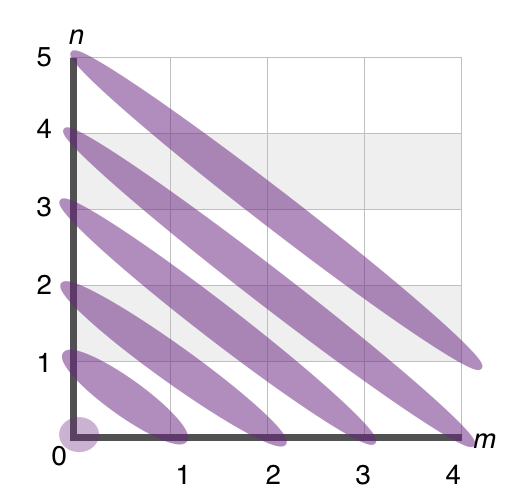
\includegraphics[height=5cm]{diagonal.png}
}%%%%% END SHIT THERE
[Caption beside object and vertically centered]{ 
Assume it does not matter in which order we add up all the terms i.e. we can add the diagonals $m+n = p$:}{fig:1}
%%%%%%%%%%%%%%%%%%%%%%%%%%%%%%


Indeed counting the terms diagonally, writing $m+n = p$: \\

\[\begin{align} \nonumber \exp(x)\exp(y) = \sum_{n=0}^{\infty}\sum_{m=0}^{\infty}\frac{x^n}{n!}\frac{y^m}{m!} &= \sum_{p=0}^{\infty}\sum_{n=0}^{p} \left(\frac{x^ny^{p-n}}{p!} \right) \\\vspace*{5pt} \nonumber
&= \sum_{p=0}^{\infty}\sum_{n=0}^{p}\left(\frac{pCn x^n y^{p-n}}{p!}\right) \\\vspace*{5pt} \nonumber
&= \sum_{p=0}^{\infty} \frac{1}{p!} \sum_{n=0}^{p} pCn x^n y^{p-n} \\\vspace*{5pt} \nonumber
&= \sum_{p=0}^{\infty} \frac{(x+y)^p}{p!} = \exp(x+y) \end{align}\]

\end{proof}

We now have $\cos and \sin$ You will prove on sheet 2 question 1 that they are $2\pi$-periodic and all the trigonmetric formulae that follow, i.e. $cos(A+B)$ etc. \textit{Remember them, or be able to derive them in 15 seconds!}\\\\

\subsektion{Other infinite series which you should know}\\

$\log(x) \neq \displaystyle{\sum_{n=0}^{\infty} a_n x^n}$ for any $a_n$ (try putting $x=0$, and you would get ``$-\infty = a_0$''...bullshit)\\

$\displaystyle{\log(1+x) = 0 + x - \frac{x^2}{2} + \frac{x^3}{3} - \frac{x^4}{4} + \dots = \sum_{n=0}^{\infty} \frac{(-1)^{n+1}x^n}{n} }$\\

$\displaystyle{\frac{1}{1+x} = 1 - x + x^2 - x^3 + x^4 + \dots = \sum_{n=0}^{\infty} x^n(-1)^n, \; |x| < 1 }$\\
This is an example of the geometric series $a + ar + ar^2 + \dots = \frac{a}{1-r}, \; |r|<1$\\

N.B. We could integrate the series for $\frac{1}{1+x}$ to obtain $\log(1+x) + c = x - \frac{1}{2}x^2 + \frac{1}{3}x^3 - \dots$ assuming integrating term by term is allowed. Letting $x = 0 \implies c = 0$\\\\

\subsubsektion{The Binomial Series}
The Geometric series is a special case of the Binomial Series:\\

$\displaystyle{(1+x)^{\alpha} = 1 + \alpha x + \frac{\alpha(\alpha -1)}{2}x^2 + \dots + \frac{\alpha(\alpha-1)\dots(\alpha-p)}{(p+1)!}x^{p+1} + \dots \quad (\alpha \in \R) }$

This series converges provided $|x|<1$. Note, if $\alpha \in \N$, then eventually the coefficients become zero and the power series \textbf{terminates} as a polynomial of degree $N$. The series then becomes the binomial theorem: $(1+x)^n = \sum_{k=0}^{n} nCk x^k$\\

Proof by: 
\begin{enumerate}
\item Leave it to M1F
\item Induction
\end{enumerate}

\vspace*{\fill}
\hfill
\begin{center}
[\textit{Lecture 8, more stuff on series... Panopto broke :S}]
\end{center}
\vspace{\fill}
\newpage

\subsektion{Maclaurin Series}

\textit{What Kind of functions have a power series?}\\
\marginnote{Lecture 9\\ 31.10.2014}[-0.5cm]

i.e. When can we write $\displaystyle{f(x) = a_0 + a_1x + a_2x^2 + \dots a_nx^n = \sum_{n=0}^{\infty} a_nx^n}$?\\

Note that if this is true then $f(0) = a_0$. So if $f(x)$ is \textbf{differentiable} (see later)  and it is legitimate to differentiate an infinite series term by term, then $f'(x) = a_1 + 2a_2 + \dots na_n = \sum_{n=0}^{\infty} na_nx^{n-1}$. Now we put $x=0$, to get $f'(0) = a_1$. \\

In general, if the function $f(x)$ can be differentiated $r$ times (and so can the series), then $f^{(r)}(0) = a_r r!x^0 + 0 + 0 + 0 + \dots \implies \boxed{a_r = \dfrac{f^{(r)}}{r!}}$\\

(if $n<r$ in sum, one of the prefactors of $x^{n-r}$ is 0. If $n>r, x^{n-r}$ is 0, when $x=0$. So only one term, $n=r$, remains.)\\

So formally, \begin{Definition} \begin{shaded} if the function has a power series then we expect the \textbf{Maclaurin Series} (or the Taylor series about $x=0$) to be:\\

$\displaystyle{f(x) = f(0) + xf'(0) + \frac{x^2f''(0)}{2!} + \dots + \frac{x^rf^{(r)}(0)}{r!} = \sum_{n=0}^{\infty} \frac{f^{(n)}(0)}{n!} x^n}$\\
\end{shaded}
\end{Definition}

We suspect therefore, the only those functions with an abitrary number of derivatives of $x=0$ have the power series expansion.\\

So $\log(x), x^{3.1}, \sin(x^{\frac{1}{2}}),$ or $|x^3|$ do not have series expansions. There are some functions for which the power series exists but converges to a different function. Such functions are called \textbf{non-analytical} functions. e.g.\\

$f(x) = \begin{cases}
 e^{-\frac{1}{x^2}} & x \neq 0\\
0 & x=0\\
 \end{cases}$\\
 
 We shall not worry about such functions anymore.\\
 
So a Maclaurin series exists $\iff f^{(n)}(0)$ exists $\forall n$\\

e.g. $f(x) = e^{-x}\sin(2x) = 2x - 2x^2 + \mathcal{O}(x^3)$\\



Next lecture we will look at the Analysis very briefly. Next term you will do it ``properly''.\\
\pagebreak
\subsektion{Key Results of Analysis}

For any power series $\displaystyle{\sum_{n=0}^{\infty} a_nx^n}$ ($a_n, x \in \mathbb{C}$), $\exists \R$ such that:

\begin{itemize}
\item if $|x| < R$ series converges
\item if $|x| > R$ series does not converge
\item if $|x| = R$ anything can happen
\item if $R = 0$ series converges only for $x = 0$
\item if ``$R = \infty$'' series converges $\forall x$
\end{itemize}

$R$ is called the \textbf{radius of convergence}:

\begin{figure}[!htb]
\centering
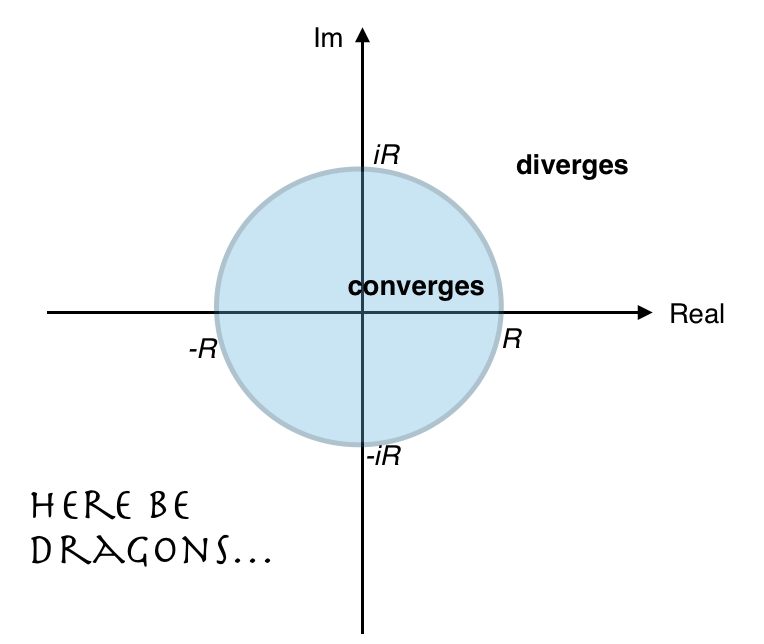
\includegraphics[height=8cm]{circle.png}
\label{fig:digraph}
\end{figure}


\begin{example}$(x+\alpha)^{\alpha} \quad a \neq 0 \in \R, \alpha \in \R$\\

$\implies a^{\alpha}(1 + \frac{x}{a})^{\alpha}$ assuming $a >0$ (otherwise if $a <0$, write $a=-b, (x-b)^{\alpha} = b^{\alpha}(\frac{x}{b} -1)^{\alpha})$\\

$= (1+t)^{\alpha}$ we ``know'' this requires $|t|<1 \implies |\frac{x}{a}| < 1 \implies |x| < |a|$, so $\boxed{R = |a|}$. \\\\ 
\end{example}

\underline{What limits the circle of convergence?}\\

In practice, the series converges in as big a circle as it can i.e. until it reaches a singular point.\\

e.g. $\frac{1}{x^2+1}$ is singular (infinite) when $x=i$, so $R \ngtr 1$ (else series would have to converge at $x = i$, but it can't as function is infinite there), so $R = 1$ for this function.




 
 





%%%%%%%%%%% Include handout
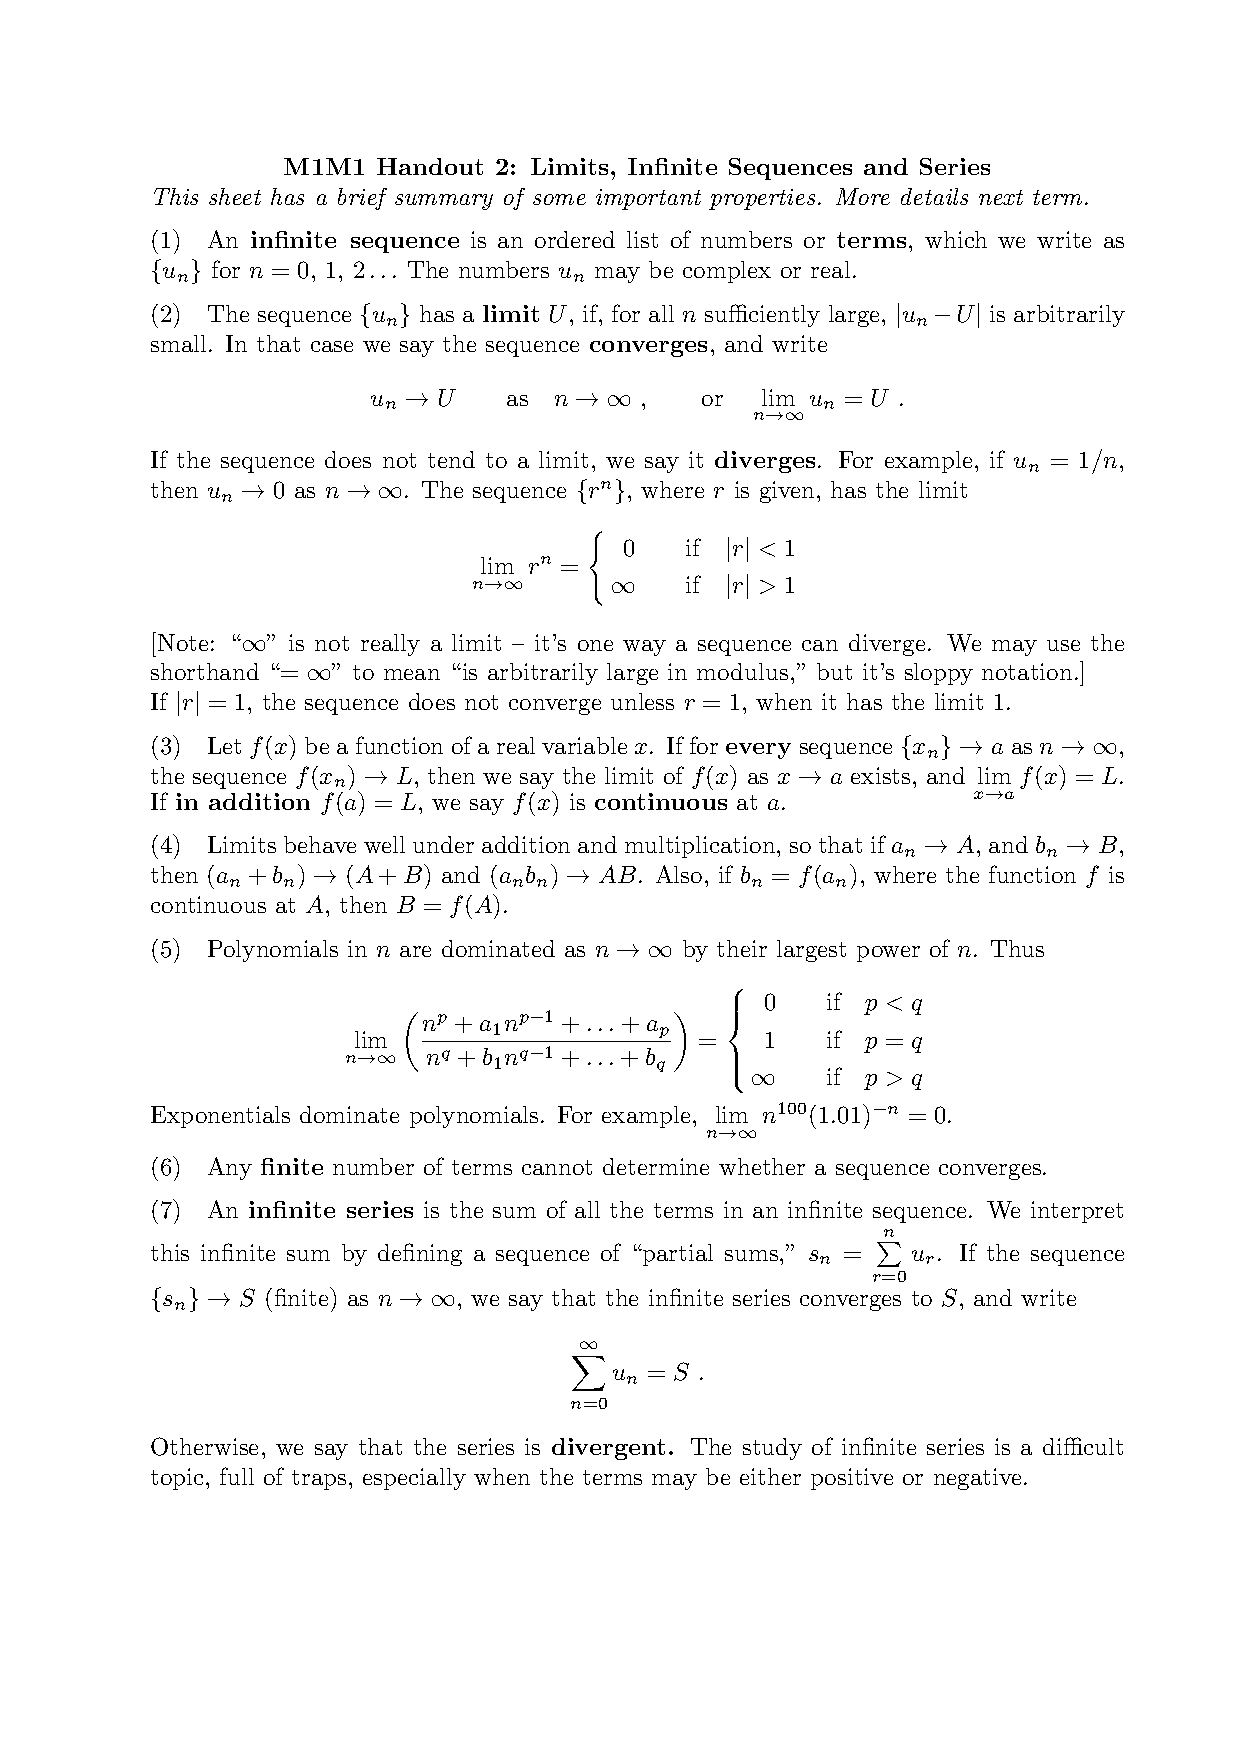
\includepdf[pages = {1,2}]{series.pdf}


\vspace*{\fill}
\hfill
\begin{center}
[\textit{Lectures 10, 11, 12 on basic analysis and differentiation, see handout and panopto}]
\end{center}
\vspace{\fill}
\newpage


\section{Differentiation}
The product rule and chain rule extend to more than two functions e.g. \marginnote{Lecture 13\\ 10.11.2014}[-0.5cm]\\


$(fgh)' = f'(gh) + f(gh)' = f'(gh) + fg'h + (fg)h'$\\

Similarly (by defining $g(h(x)) \equiv k(x)$):\\
 $f[g(h[x])]' = f[k(x)]' = f'(k(x)).k'(x) = f'(g(h(x)))g'(h(x))h'(x)$\\
 
 It's easier to just remember that:\\
 
 $\displaystyle{
 \frac{dy}{dx} = 
 \frac{dy}{du}
 \frac{du}{dt}
 \frac{dt}{d\Omega}
 \frac{d\Omega}{d\chi}
 \frac{d\chi}{d\xi}
 \frac{d\xi}{dx}   
 }$ etc.\\
 
\subsektion{``First Principles'' differentiation}

What is $\dfrac{\mathrm{d}}{\mathrm{d}x} (e^x)$?\\

= $\displaystyle{
\lim_{\epsilon \to 0} 
\left(\dfrac{e^{x + \epsilon} - e^x}{\epsilon}\right) 
= e^x \lim_{\epsilon \to 0}
\left(\frac{e^x - 1}{\epsilon}\right) 
= e^x \lim_{\epsilon \to 0} 
\left(\frac{1 + \epsilon + \mathcal{O}(\epsilon ^2) -1}{\epsilon} \right) 
}$\\

= $\displaystyle{
e^x \lim_{\epsilon \to 0} 
[1 + \mathcal{O}(\epsilon)] = e^x
}$\\\\

\textbf{Excerise}: Show that $\dfrac{dx}{dx} = 1$ from first principles\\

So $1 = \dfrac{dx}{dx} = \dfrac{dx}{dy}\dfrac{dy}{dx}$ (using chain rule). i.e. $\boxed{\dfrac{dy}{dx} = \dfrac{1}{dx/dy}}$\\\\


N.B. Next term you will meet partial derivatives, $\frac{\partial u}{\partial x}$; The chain rule for partial differentiation is more complicated, and $\frac{\partial u}{\partial x} \neq \frac{1}{\partial x / \partial u}$ necessarily.\\\\

\subsubsektion{Inverse Functions}

\textit{If $y = \log x$, What is $\dfrac{dy}{dx}$?}\\

Write $x = e^y \implies \dfrac{dx}{dy} = e^y \implies \dfrac{dy}{dx} = \dfrac{1}{e^y} = \dfrac{1}{x}$\\\\

\textit{What is $\dfrac{\mathrm{d}}{\mathrm{d}x} (\sin^-1 x)$?}\\

$\dfrac{dx}{dy} 
= \dfrac{d}{dy}(\sin y) 
= \dfrac{d}{dy}
\left[y - \dfrac{y^3}{6} + \dfrac{y^5}{120} + \dots \dfrac{y^n}{n!}\right] 
= \left[1 - \dfrac{y^2}{2} + \dfrac{y^4}{24} + \dots\right]
= \cos y
$\\

Or we could use first principles:

\[\begin{align} \nonumber \frac{d}{dy}[\sin y] 
= \lim_{\epsilon \to 0}
\left[\frac{\sin(y+\epsilon) - \sin(y)}{\epsilon} \right]
&=\lim_{\epsilon \to 0}
 \left[\frac{\sin y \cos \epsilon + \sin \epsilon \cos y - \sin y}{\epsilon} \right] 
 \\ \nonumber
&= \lim_{\epsilon \to 0}
\left[\frac{\sin \epsilon}{\epsilon}\cos y\right]
+ \lim_{\epsilon \to 0}
\left[\sin y \left(\frac{\cos \epsilon -1}{\epsilon} \right) \right]
\\ \nonumber
&=\lim_{\epsilon \to 0}
\left[\frac{\epsilon + \mathcal{O}(\epsilon^3}{\epsilon} \right]\cos y
+ \sin y \lim_{\epsilon \to 0}
\left[\frac{1-\frac{\epsilon^2}{2} + \mathcal{O}(\epsilon^4) -1}{\epsilon}\right]
\\ \nonumber
&= \cos y
\end{align}
\]

Similarly $\dfrac{d}{dx}(\cos x) = -\sin x$.\\\\

$\displaystyle{
\dfrac{d}{dx}(\tan x) = \left(\frac{\sin(x)}{\cos(x)}\right) = 1 + \frac{sin^2x}{\cot x} = \frac{cos^2x + sin^2x}{\cos^2x} = \frac{1}{cos^2x} = \sec^2x
}$\\\\

Return to $\dfrac{d}{dx}(\sin^{-1}x); \quad x = \sin y$\\

$\dfrac{dx}{dy} = \cos y = \sqrt{1 - \sin^2y} = \sqrt{1 - x^2}$\\

Hence $\dfrac{dy}{dx} = \dfrac{1}{\sqrt{1-x^2}} = \dfrac{d}{dx}[\sin^{-1}x]$\\\\

\textbf{Exercise} Show $\dfrac{d}{dx}(\cos x) = -\dfrac{1}{\sqrt{1-x^2}}$\\

Hence $\dfrac{d}{dx}[\sin^{-1}x + \cos^{-1}x] = 0$, which is clear from the right angled triangle.\\
Since $\alpha = \sin^{-1}x$ and $\beta = \cos^{-1}x$, $\alpha + \beta = \frac{\pi}{2}$, obviously $\frac{d}{dx} \frac{\pi}{2} = 0$
\\

%%%%%%%%%%%%%%%%%%%%%%%%%%%%%%% Right Angled Triangle
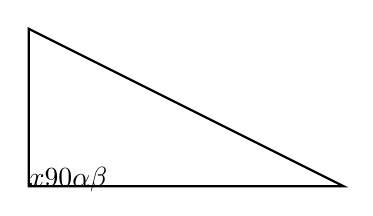
\begin{tikzpicture}[thick]
\coordinate (O) at (0,0);
\coordinate (A) at (4,0);
\coordinate (B) at (0,2);
\draw (O)--(A)--(B)--cycle;

\tkzLabelSegment[below=2pt](O,A){}%{\textit{adjacent leg}}
\tkzLabelSegment[left=2pt](O,B){\textit{$x$}}
\tkzLabelSegment[above right=2pt](A,B){\textit{1}}

\tkzMarkRightAngle[fill=orange,size=0.6,opacity=.4](A,O,B)% square angle here
\tkzLabelAngle[pos = 0.35](A,O,B){~$90\degree$}

\tkzMarkAngle[fill= orange,size=0.8cm,%
opacity=.4](B,A,O)
\tkzLabelAngle[pos = 0.6](B,A,O){$\alpha$}

\tkzMarkAngle[fill= orange,size=0.7cm,%
opacity=.4](O,B,A)
\tkzLabelAngle[pos = 0.5](O,B,A){$\beta$}

\end{tikzpicture}
%%%%%%%%%%%%%%%%%%%%%%%%%%%%%%%%%%

\subsubsektion{Logarithmic Derivative}

$\displaystyle{
\frac{d}{dx}(\log(u(x))) = \frac{d}{du}\log u.\frac{du}{dx} = \frac{1}{u}u'
}$\\

This is called a logarithmic derivative. Useful when performing integration e.g.\\

$\displaystyle{
I = \int \frac{e^x + \cos x}{1 + e^x + \sin x} \, \mathrm{d}x
}$\\

Observe that $u = 1 + e^x + \sin x$ and $u' = e^x + \cos x \implies I = \log(1 + e^x + \sin x) + c$

\pagebreak

\subsubsektion{Implicit Differentiation}

If $y$ is given implicitly in terms of $x$ e.g. $y + \tan y = x$, we can differentiate the entire equation term by term with respect to $x$:

\[\begin{flalign}\nonumber
\frac{d}{dx}(y + \tan y) = \dfrac{d}{dx}(x) &= 1
\\ \nonumber 
\implies \frac{dy}{dx}\frac{d}{dy}(y + \tan y) &= 1
\\ \nonumber
\implies \frac{dy}{dx}(1 + \sec^2y) &= 1
\\ \nonumber
\implies \frac{dy}{dx} &= \frac{1}{\sec^2y + 1} = \frac{1}{2 + \tan^2y} = \frac{1}{2 + (x-y)^2}
\end{flalign}
\]

\subsubsektion{Higher Derivatives}

If $f(x)$ is differentiable in $(a,b) \iff f'(x)$ is defined on $(a,b)$.\\

 Maybe $f'$ is also differentiable. If so, we write it as $f''$ or $\dfrac{d^2f}{dx^2}$ or $\left(\dfrac{d}{dx}\right)^2f$\\
 
 BUT NOT EVER EVER $\left(\dfrac{df}{dx}\right)^2$\\
 
 Continuing, we can write the n'th derivative (if it exists) as $f^{(n)}(x)$ or  $\dfrac{d^nf}{dx^n} $ or $\left(\dfrac{d}{dx}\right)^n f$.\\
 These forms are useful for Taylor / Maclaurin series.

\subsektion{Leibniz' Rule}

\textit{How can we (easily) differentiate a product many times?}\\

Suppose $f$ and $g$ are differentiable an arbitrarily number of times. What is $(fg)'$? Use the product rule:\\

$(fg)' = f'g + fg'$\\
$(fg)'' = (f'g + fg')' = (f'g)' + (fg')' = f''g + 2f'g' + fg''$\\
$(fg)''' = f'''g + 3f''g' + 3f'g'' + fg'''$\\

We spot a pattern, and make an inspired (but intelligent) guess:\\

$\displaystyle{
(fg)^n = \sum_{r=0}^n {n \choose k} f^{(r)}g^{(n-r)}
} \quad \} \text{ Leibniz' Formula } \quad (*)$\\\\

This is very similar to the binomial theorem:\\
$\displaystyle{
(f+g)^n = \sum_{r=0}^n {n \choose k} f^{r}g^{n-r}
}$ (which I had hoped would have been proved in M1F)\\


\begin{proof}
Use induction to prove $(*)$\\

(A) Take $n = 1: (fg)' = f'g + fg'$ by product rule, so true for $n=1$\\\\

(B) Assume $(*)$ holds when $n=k$, and try to prove it then holds for $n = k + 1$. Hence:\\

$(fg)^{(k)} = \displaystyle{\sum_{r=0}^{k}{k \choose r}f^{(r)}g^{(k-r)} }$, and differentiate again:\\

$\implies (fg)^{(k+1)} = \displaystyle{\sum_{r=0}^{k}{k \choose r} \left[f^{(r+1)}g^{(k-r)} + f^{(r)}g^{(k-r+1)} \right] }$\\

$ = \displaystyle{
f^{(s)}g^{(k+1-s)}\left[{k \choose s-1} + {k \choose s}\right]
}$\\\\

Lemma\footnote{\textit{proof}: A) Pester Alessio, B) Pester Emma, C) Use Pascal's Triangle, D) Use Factorials}: $\displaystyle{ {k \choose s-1} + {k \choose s} = {k+1 \choose s} }$\\

Assuming lemma, we obtain: $(fg)^{(k+1)} = \displaystyle{\sum_{s=0}^{k+1}{k+1 \choose s}f^{(s)}g^{(k+1-s)} }$, as required. \\

(C) Hence by induction $(*)$ holds for all natural $N$\\
\end{proof}

Note: Leibniz is very useful is one of the functions $\omega \log$ $f$ is a polynomial, as then the high derivatives vanish (are zero)\\

\begin{example} What is $\dfrac{d}{dx}(x^2\sin x)$?\\

Using Leibniz, $f = \sin x, g = x^2$:

\[\begin{flalign} \nonumber 
\dfrac{dy}{dx} &= (\sin x)^{(100)}x^2 + {100 \choose 1}\sin x^{(99)}.2x + {100 \choose 2}\sin x^{(98)}.2 + 0 + 0 + \dots 
\\ \nonumber
&= \sin x[x^2 -9900] - 200x\cos x
\end{flalign}\]\\
\end{example}

\begin{example}: What is the Maclaurin series for $y = \sin^{-1}x$?\\

$y' = \dfrac{1}{\sqrt{1-x^2}}, y'' = x(1-x^2)^{-3/2}$\\

$\implies (1-x^2)y'' = xy'$\\

Differentiate entire equation $n$ times using Leibniz rule:\\

$\displaystyle{
[(1-x^2)y'']^{(n)} = [xy']^{(n)} = xy^{(n+1)} + ny^{(n)}
}$\\

Note that:
$\displaystyle{
[(1-x^2)y'']^{(n)} = (1-x^2)y^{(n+2)} + n(2x)y^{(n+1)} + \frac{n(n-1)}{2}(-2)y^{(n)}
}$\\

Hence $(1-x^2)y^{(n+2)} - (2n+1)xy^{(n+1)} - n^2y^{(n)} = 0$\\

So at $x = 0$, we have:\\
$y^{(n+1)}(0) = n^2y^{(n)}(0) \quad \forall n$\\

Now $y = \sin^{-1}x \implies y(0) = 0$, and $y' = \dfrac{1}{\sqrt{1-x^2}} \implies y'(0) = 1$\\
Means all even derivatives are zero.\\

$y^{(3)}(0) = 1, y^{(5)}(0) = 3^2, y^{(7)}(0) = 5^2.3^2$\\

So $\displaystyle{
\sin^{-1}x = \sum_{n =0}^{\infty} \frac{x^{2n+1}}{(2n+1)!}(n-2)^2(n-4)^2 \dots 5^2 \times 3^2 \times 1 
}$

\end{example}
